\chapter{Introduzione}

\section{Prima Lezione}
Un Sistema Operativo (SO) agisce come intermediario tra l'utente e l'hardware, fornendo gli strumenti per un uso corretto delle risorse della macchina (CPU, memoria, periferiche). Ha due obiettivi principali:
\begin{itemize}
    \item Dal punto di vista dell'utente: rendere il sistema facile da usare.
    \item Dal punto di vista della macchina: ottimizzare l'uso delle risorse in modo sicuro ed efficiente.
\end{itemize}

\subsection{Architetture Single/Multi-Core}
Negli anni 2000 si è passati da processori single-core a multi-core, con CPU dotate di più core in grado di eseguire istruzioni di programmi diversi simultaneamente. La figura \ref{fig:multi-core} illustra una tipica architettura dual-core.

\begin{figure}[h!]
    \centering
    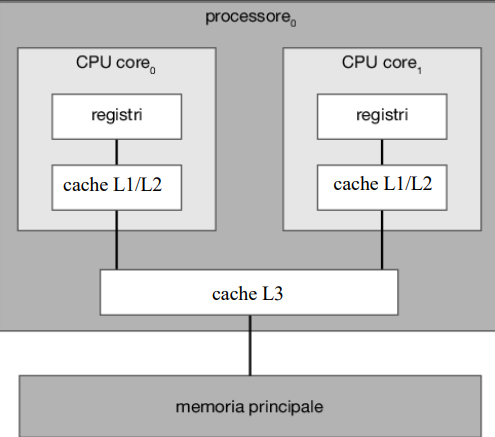
\includegraphics[width=0.5\textwidth]{1/multi-core-architecture.png}
    \caption{Architettura di un processore dual-core}
    \label{fig:multi-core}
\end{figure}

\subsection{Gestione delle Interruzioni}
Il SO è un sistema ``event-driven'', ossia viene attivato quando si verificano eventi come \textit{interrupt} (hardware) o \textit{eccezioni} (software). Ogni interruzione attiva una porzione specifica di codice del SO. La figura \ref{fig:interrupt-handler} rappresenta un esempio di gestione delle interruzioni.


\subsection{Memoria e Cache}
La gerarchia delle memorie include registri, cache, RAM e memoria secondaria. I dati più frequentemente utilizzati vengono spostati in memorie più veloci, come la cache. In figura \ref{fig:memory-hierarchy} si può osservare la gerarchia delle memorie.

\begin{figure}[h!]
    \centering
    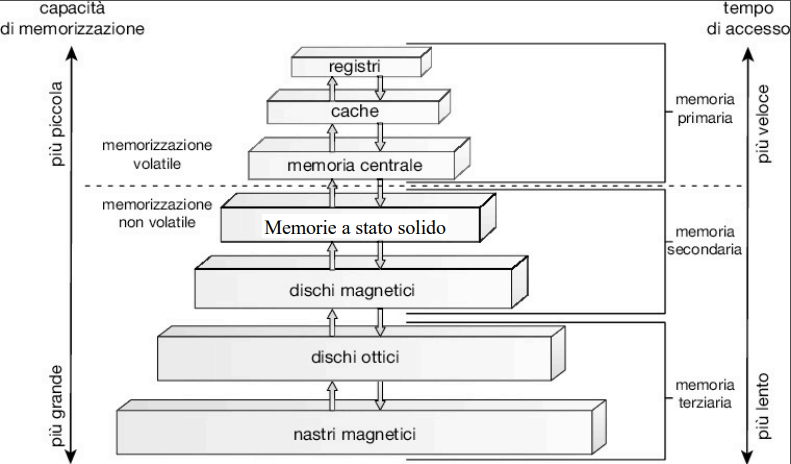
\includegraphics[width=0.5\textwidth]{1/memory-hierarchy.png}
    \caption{Gerarchia delle memorie}
    \label{fig:memory-hierarchy}
\end{figure}

\section{Multitasking e Time-sharing}
Il SO gestisce più programmi contemporaneamente, assegnando la CPU a ciascuno quando disponibile. Il time-sharing permette di distribuire il tempo della CPU tra più utenti, dando l'impressione di simultaneità.

\section{Protezione della Memoria}
Il SO protegge la memoria primaria da accessi non autorizzati attraverso il meccanismo di registri base e limite, come mostrato in figura \ref{fig:memory-protection}.
